
% !TeX spellcheck = ptBR
% !TeX encoding = utf8
% !TeX program = lualatex
% -----------------------------------
\documentclass[
% -- op\c{c}ões da classe memoir --
article,			                                    % indica que é um artigo acadêmico
12pt,				                                   % tamanho da fonte
oneside,											% para impressão apenas no recto. Oposto a twoside
a4paper,											% tamanho do papel. 
% -- op\c{c}ões da classe abntex2 --
%chapter=TITLE,								  % títulos de capítulos convertidos em letras maiúsculas
section=TITLE,									 % títulos de se\c{c}ões convertidos em letras maiúsculas
%subsection=TITLE,							% títulos de subse\c{c}ões convertidos em letras maiúsculas
%subsubsection=TITLE % títulos de subsubse\c{c}ões convertidos em letras maiúsculas
% -- op\c{c}ões do pacote babel --
english,											% idioma adicional para hifeniza\c{c}ão
brazil,												% o último idioma é o principal do documento
sumario=tradicional
]{ltxdoc}

%\usepackage[top=120pt, bottom=2.5cm, left=3cm, right=2cm, headheight=95pt, footskip=66pt]{geometry}%
% PACOTES
%!TEX root = PREAMBULO.tex
\usepackage{lmodern}			% Usa a fonte Latin Modern			
\usepackage[T1]{fontenc}		% seleção de códigos de fonte.
\usepackage[utf8]{inputenc}		% determina a codificação utiizada (conversão automática dos acentos)
\usepackage{hyperref}  			% controla a formação do índice
\usepackage{parskip}			% espaçamento entre os parágrafos
\usepackage{microtype} 			% para melhorias de justificação
\usepackage{morefloats}			% permite mais floats
\usepackage{indentfirst} % identar o  primeiro paragrafo
\usepackage{lipsum}  % textos exparsos
% Babel e ajustes
\usepackage[brazil]{babel}		% idiomas
\addto\captionsbrazil{
	%% ajusta nomes padroes do babel
	\renewcommand{\bibname}{Refer\^encias}
	\renewcommand{\indexname}{\'Indice}
	\renewcommand{\listfigurename}{Lista de ilustra\c{c}\~{o}es}
	\renewcommand{\listtablename}{Lista de tabelas}
	%% ajusta nomes usados com a macro \autoref
	\renewcommand{\pageautorefname}{p\'agina}
	\renewcommand{\sectionautorefname}{se{\c c}\~ao}
	\renewcommand{\subsectionautorefname}{subse{\c c}\~ao}
	\renewcommand{\paragraphautorefname}{par\'agrafo}
	\renewcommand{\subsubsectionautorefname}{subse{\c c}\~ao}
	\renewcommand{\paragraphautorefname}{subse{\c c}\~ao}
}  

\usepackage{color}
 

% COMANDOS PROPRIOS
\newcommand{\abnTeX}{abn\TeX}
\newcommand{\abnTeXForum}{\url{http://groups.google.com/group/abntex2}}
\newcommand{\abnTeXSite}{\url{http://www.abntex.net.br/}}

\title{\textbf{A classe \textsf{abntex2}}: \\ \Large{Documentos
		técnicos e científicos brasileiros \\compatíveis com as normas ABNT}}

%   \thanks{Este documento
	%   se referete ao \textsf{abntex2} versão \fileversion,
	%   de \filedate.}

 


\EnableCrossrefs
\CodelineIndex
\RecordChanges

\changes{v1.0}{2013/02/01}{Versão inicial}
\changes{v1.9.3}{2015/01/26}{Release 1.9.3}
\changes{v1.9.4}{2018/06/06}{Release 1.9.4}

\usepackage[fontsize=12pt]{scrextend}
\usepackage{backref}
\usepackage{lastpage}     % para conseguir identificar a quantidade de páginas no preâmbulo
\usepackage{fancyhdr} 		    % para incluir headings e footers
% ------------------------------------------------------
\usepackage{fontspec} %% => Ligar fonte Arial
\setmainfont{Arial}
\usepackage{fontspec} %% => Ligar fonte Arial
\setmainfont{Arial}
% ------------------------------------------------------  													% Trazer os pacotes
%!TEX root = preambulo.tex
% ---
% Pacotes de citações
% ---
%\usepackage[brazilian,hyperpageref]{backref}	 % Paginas com as citações na bibl
\usepackage[alf, % Permite ficar em ordem alfabetica
abnt-repeated-author-omit=true,  % Omitir autores com o mesmo nome
abnt-emphasize=bf, %Nome em destaque em negrito
abnt-etal-list=0, % utilizar o parentese em luga do colchete
]{abntex2cite}	% Citações padrão ABNT
\usepackage{nomencl} 			% Lista de simbolos
\usepackage{color}				% Controle das cores
\usepackage{nomencl} 			% Lista de simbolos
\usepackage{color}				% Controle das cores
\usepackage{graphicx,subcaption}		% Inclusão de gráficos
\usepackage{float} % Força o posicionamento da figura
\usepackage{microtype} 			% para melhorias de justificação
% ---
\usepackage{wrapfig}
\usepackage{blindtext} % Para gerar comentarios
\usepackage{tikz}
\usetikzlibrary{calc,positioning,arrows,shapes,shadows,fit,patterns,quotes,spy}
\usepackage{quoting}
\usepackage{setspace} % Este pacote altera o espaçamento entre linhas
\usepackage{amsmath} % modo matematico
% ---
\usepackage{todonotes} % Para comentarios magicos
\usepackage{comment}
\usepackage{verbatim}  % Comentários em multilinhas
\usepackage{listings}

\usepackage{xcolor} % Para cores personalizadas

\definecolor{keywords}{RGB}{255,0,90}
\definecolor{comments}{RGB}{0,0,113}
\definecolor{red}{RGB}{160,0,0}
\definecolor{green}{RGB}{0,150,0}
\definecolor{codegreen}{rgb}{0,0.6,0}
\definecolor{codegray}{rgb}{0.5,0.5,0.5}
\definecolor{codepurple}{rgb}{0.58,0,0.82}
\definecolor{backcolour}{rgb}{0.95,0.95,0.92}
\lstdefinestyle{mystyle}{
	backgroundcolor=\color{backcolour},   
	commentstyle=\color{codegreen},
	keywordstyle=\color{magenta},
	numberstyle=\tiny\color{codegray},
	stringstyle=\color{codepurple},
	basicstyle=\ttfamily\footnotesize,
	breakatwhitespace=false,         
	breaklines=true,                 
	captionpos=b,                    
	keepspaces=true,                 
	numbers=left,                    
	numbersep=5pt,                  
	showspaces=false,                
	showstringspaces=false,
	showtabs=false,                  
	tabsize=2
}
\lstset{style=mystyle}
\usepackage[framemethod=TikZ]{mdframed}
\mdfdefinestyle{MyFrame}{%
	linecolor=blue,
	outerlinewidth=2pt,
	roundcorner=20pt,
	innertopmargin=\baselineskip,
	innerbottommargin=\baselineskip,
	innerrightmargin=20pt,
	innerleftmargin=20pt,
	backgroundcolor=gray!40!white}


% ------------------------------------------------------ 												% Trazer os pacotes
\usepackage{geometry}
\geometry{top=110pt, bottom=3.5cm, left=3.0cm, right=2.0cm, headheight=70pt}
\usepackage[utf8]{inputenc}
\usepackage{babel}
\usepackage[T1]{fontenc}
\usepackage{wrapfig,lipsum,booktabs}
\usepackage{graphicx}
\usepackage{fancyhdr}
\pagestyle{fancy}
\usepackage{tikz}
\usetikzlibrary{calc,positioning,arrows,shapes,shadows,fit,patterns,quotes,spy}
\usepackage{supertabular}  % Ppara tabelas em varias paginas
\usepackage{tabularx}
\usepackage{longtable}
\usepackage{pdflscape}
\usepackage[fontsize=12pt]{scrextend}
%%%%%%%%%%%%%
\usepackage{multirow}
\usepackage{setspace}                                                        % Para espacamentos
\usepackage{varioref}                                                           % referencia cruzada
\usepackage{enumitem}  													% para melhoria nos itens numerados
\usepackage{xcolor} 															% Para cores personalizadas
\usepackage{wrapfig}
\usepackage{float} 								% Força o posicionamento da figura
\usepackage[]{backref}	                         %  VOLTAR com as citações
\usepackage{hypernat}
\usepackage{etoolbox}
%\usepackage{threeparttable} 
\usepackage[flushleft]{threeparttablex}
\usepackage{booktabs}
\usepackage{multirow}
 												% Trazer os pacotes
%%%CONFIGURACOES
\setlength{\parindent}{0cm} % SEM IDENTECAO

 
% alterando o aspecto da cor azul
\definecolor{blue}{RGB}{41,5,195}
% informações do PDF
\makeatletter
\hypersetup{
	pagebackref=true,
	pdftitle={\@title}, 
	pdfauthor={\@author},
	pdfsubject={Modelo de artigo científico com abnTeX2},
	pdfcreator={LaTeX with abnTeX2},
	pdfkeywords={abnt}{latex}{abntex}{abntex2}{atigo científico}, 
	colorlinks=true,       		% false: boxed links; true: colored links
	linkcolor=blue,          	% color of internal links
	citecolor=blue,        		% color of links to bibliography
	filecolor=magenta,      		% color of file links
	backref=page,           % Para back ref
	urlcolor=blue,
	bookmarksdepth=4
}
\makeatother
%--
% O tamanho do parágrafo é dado por:
\setlength{\parindent}{1.25cm}
\usepackage{threeparttable} 
% Controle do espaçamento entre um parágrafo e outro:
\setlength{\parskip}{0.1cm}  % tente também \onelineskip

% Espaçamento simples
%\SingleSpacing

% Configurações do pacote backref
% Usado sem a opção hyperpageref de backref
\renewcommand{\backrefpagesname}{Citado na(s) página(s):~}
% Texto padrão antes do número das páginas
\renewcommand{\backref}{}
% Define os textos da citação
\renewcommand*{\backrefalt}[4]{
	\ifcase #1 %
	Nenhuma citação no texto.%
	\or
	Citado na página #2.%
	\else
	Citado #1 vezes nas páginas #2.%
	\fi}%

%--
  
\setlength{\parindent}{0cm} % SEM IDENTECAO


%\renewcommand{\footrulewidth}{1pt}

%\geometry{a4paper, includehead, top=-0.4cm, left=2cm}
\setlength\headwidth{\paperwidth}
\fancyhead{} % Limpar all fields cabecalho
\fancyfoot{} % Limpar all fields rodape
\pagestyle{fancyplain}                    % aplicando o estilo 
\fancyhfoffset[L]{0.2cm}\fancyhfoffset[R]{0.2cm}

\chead{
\includegraphics[width=\headwidth]{pre-pos-textuais/cabecalho}}
\renewcommand{\headrulewidth}{0pt}

%\clearpage\begingroup\pagestyle{empty}\cleardoublepage\endgroup

\usepackage{lastpage} % number of last page 
\rfoot{Page \thepage\ de \pageref{LastPage}}
\cfoot{
\includegraphics[width=0.8\headwidth]{pre-pos-textuais//rodape}}

\renewcommand{\footrulewidth}{0pt} 
\renewcommand{\headrulewidth}{0pt}
\usepackage{lastpage} % number of last page 
\rfoot{ \thepage\ de \pageref{LastPage}}


\makeatletter
\patchcmd{\BR@backref}{\newblock}{\newblock(~}{}{}
\patchcmd{\BR@backref}{\par}{)\par}{}{}
\makeatother

\renewcommand{\backrefxxx}[3]{(page \hyperlink{page.#1}{#1})} 
% ------------------------------------------------------
\usepackage{fontspec} %% => Ligar fonte Arial
\setmainfont{Arial}
\usepackage{fontspec} %% => Ligar fonte Arial
\setmainfont{Arial}
% ------------------------------------------------------ 

\begin{document}
\maketitle
\thispagestyle{empty} % Não enumere esta pagina-
 

%\tableofcontents

%\listoftables
 
%!TEX root = ..//Avali-Arena-Esportivas.tex
 
\begin{center}
	\textbf{XXIII COBREAP - CONGRESSO BRASILEIRO DE ENGENHARIA DE AVALIAÇÕES E PERÍCIAS - JOÃO PESSOA - 2025}
\end{center}
\begin{center}
	\textbf{TRABALHO DE AVALIAÇÃO}
\end{center}

Avaliação de arena esportiva pelo método comparativo direto de dados de mercado, com a aplicação do tratamento científico\\ 
RESUMO\\ 
Arenas esportivas são locais multifuncionais projetados para sediar uma variedade de eventos, incluindo competições esportivas, shows, conferências, futebol e outros tipos de entretenimento.\\ 


Este trabalho pretende de forma objetiva e tão simples quanto possível, estabelecer uma marcha numérica baseada através da Inferência estatística, pelo Método Direto Comparativo de Dados de Mercado - MDCDM, com o conhecimento técnico da engenharia de avaliações, mostrando que estes espaços podem ser avaliados por ele.\\ 
Palavras-chave: Ativos singulares, Arenas poliesportivas, Futebol

% ------
 
\newpage
% ------
%!TEX root = ..//preambulo.tex

\section{Introdução}

\hspace*{1.25 cm} O rompimento da barragem de Fundão, no povoado de Bento Rodrigues, município de Mariana, Minas Gerais, em 5 de novembro de 2015, lançou rejeitos de mineração de ferro na bacia hidrográfica do Rio Doce, causando uma série de prejuízos, incluindo perdas de vidas humanas e contaminação ambiental a jusante do corpo hídrico. \\
%
\hspace*{1.25 cm} O volume de rejeitos liberado, contendo material estranho ao bioma característico da região, alterou simultaneamente as condições dos corpos hídricos e da vegetação marginal..\\
%
\hspace*{1.25 cm}A cobertura desse evento foi amplamente noticiada pela imprensa nacional e internacional, incluindo veículos como \textit{The Wall Street Jornal}, \textit{The Guardian}, \textit{Le Monde}, entre outros.\\
%
\hspace*{1.25 cm} Em acordo com o Ministério publico (MP) e sua controladora a anglo-australiana  \textit{BHP Billinton} ,  baseado nos princípios de poluidor pagador, trazidos no artigo 3º, inciso IV, da Lei 6.938/81 (Politica Nacional do Meio Ambiente), estabeleceram um termo de pactuação e posterior outra repactuação.  A repactuação atendendo o principio do poluidor-pagador, visa o dever de corrigir, recuperar e/ou eliminar os efeitos negativos ja produzidos em uma contaminação antrópica. \\
% 
\hspace*{1.25 cm}  A repactuação, utilizando ferramentas de cartografia , acordo com \cite[p~79]{Magri}, determinando ações de reparação aos atingidos e a  amplitude de localização geográfica em que ocorram ações de contaminação, e  por meio de direta interveniência  judicial e administrativa, e a fundação criada para reparação do rio Doce, denominada Fundação Renova.\\
 %
\hspace*{1.25 cm} Passados nove anos, com base na data de 23 de maio de 2025, e com a redução da atenção midiática sobre o desastre, este estudo propõe como objeto de pesquisa avaliar se os efeitos da contaminação por rejeitos ainda podem ser detectados por sensores orbitais e se há alterações passíveis de observação por esses instrumentos. Esses aspectos são objetos de perícia ambiental, conforme descrito por Arantes (p. 130). \cite[p.130]{Arantes} \\
 %
\hspace*{1.25 cm}  A justificativa deste estudo fundamenta-se na delimitação estabelecida pela repactuação entre o Ministério Público e a Fundação Renova. Além disso, considera-se a análise dos enquadramentos dos corpos d’água e as diretrizes ambientais previstas na Resolução Conama nº 357, de março de 2005, alterada pelas Resoluções nº 410/2009 e nº 430/2011, que podem ser observadas em locais dentro e fora do âmbito da repactuação.\\
%
\hspace*{1.25 cm} A tragédia do rompimento da barragem de Fundão, em Mariana/MG, ocorrida em 5 de novembro de 2015, representa um dos maiores desastres socioambientais do Brasil. Este evento catastrófico lançou aproximadamente 39 milhões de metros cúbicos de rejeitos de mineração na Bacia do Rio Doce, causando a perda de 19 vidas e impactando severamente populações em dezenas de municípios até a foz no Espírito Santo. A amplitude do desastre e seus prejuízos humanos e ambientais ganharam notoriedade na imprensa nacional e internacional, como The Wall Street Journal, The Guardian e Le Monde.\\
%
\hspace*{1.25 cm} Em resposta à calamidade, as partes envolvidas – a Samarco, suas acionistas Vale e BHP Billiton, a União e os governos de Minas Gerais e do Espírito Santo – firmaram o Termo de Transação e Ajustamento de Conduta (TTAC) em 2 de março de 2016. Com base neste acordo, foi criada a Fundação Renova em 2016, uma entidade privada com a missão de conduzir as 42 ações e programas socioeconômicos e socioambientais definidos para a reparação. No entanto, ao longo dos anos, a atuação da Fundação Renova foi alvo de diversas críticas e gerou um passivo significativo de 85 mil processos judiciais, evidenciando a necessidade de uma solução mais eficaz e abrangente.\\
%
\hspace*{1.25 cm} Diante da complexidade e da insatisfação com o progresso reparatório, iniciaram-se em março de 2021 as tratativas para uma renegociação ampla dos acordos, formalizadas pela Carta de Premissas em 22 de junho de 2021. Este processo, conduzido inicialmente pelo Conselho Nacional de Justiça (CNJ) e, a partir de agosto de 2022, sob a liderança do Tribunal Regional Federal da 6ª Região (TRF6) através da Mesa de Repactuação, buscou encerrar os múltiplos litígios por meio de um procedimento de conciliação. Após quase três anos de intensas negociações, o Acordo Judicial para Reparação Integral e Definitiva Relativa ao Rompimento da Barragem de Fundão foi finalmente assinado em Brasília em 25 de outubro de 2024 e homologado por unanimidade pelo Supremo Tribunal Federal (STF) em 6 de novembro de 2024.\\
%
\hspace*{1.25 cm} Este novo acordo, que substitui integralmente o TTAC de 2016 e seus aditivos, busca a reparação integral e definitiva de todos os danos socioambientais e socioeconômicos. Um dos seus pilares é a extinção da Fundação Renova e do Comitê Interfederativo (CIF), transferindo a responsabilidade integral pelas ações de reparação diretamente para a Samarco, que iniciará um período de liquidação para essa transição. O acordo prevê um valor econômico total de R\$ 170 bilhões, que inclui:
\begin{description} [itemsep=1pt,parsep=1pt]\vspace{0.00mm} 
	\item[•] R\$ 38 bilhões já desembolsados desde a tragédia.
	\item[•] R\$ 100 bilhões em "dinheiro novo", destinados aos entes públicos para custeio de medidas compensatórias e projetos socioambientais e socioeconômicos.
	\item[•] R\$ 32 bilhões em "Obrigações de Fazer", que incluem indenizações individuais, reconstrução de comunidades e recuperação de áreas degradadas, sem um teto financeiro pré-determinado, devendo a Samarco comprovar a conclusão de cada obrigação.
\end{description}

\hspace*{1.25 cm}
A nova governança do processo reparatório será marcada pela transparência, com a criação de um "Portal Único" denominado "Reparação Rio Doce", onde todas as partes envolvidas (signatários) serão responsáveis pela atualização dos dados, permitindo à sociedade civil acompanhar detalhadamente a implementação do acordo. A homologação do acordo também resultará na extinção de inúmeras ações judiciais e procedimentos administrativos, visando a definitiva resolução dos litígios.

\hspace*{1.25 cm} Com base na exposição acima, as seguintes hipóteses são formuladas:
\begin{description} [itemsep=1pt,parsep=1pt]\vspace{0.00mm} 
	\item[$H_{1}$:\label{h1}] O sensor orbita Landsat 8 consegue identificar alterações em respostas em radiância na época  do ocorrido, e seus efeitos ainda podem ser mensurados
	\item[$H_{2}$:\label{h2}] Se este sensor orbital consegue distinguir alterações espectral  do fenômeno, o mesmo consegue determinar sua amplitude espacial geográfica.
	\item[$H_{3}$:\label{h3}] Existe resquícios desta contaminação no local, e que podem ser mensurados.
\end{description}

% ------
%!TEX root = ..//Avali-Arena-Esportivas.tex
\section{ AMOSTRA }

\hspace*{1.25 cm} A amostra adotada neste estudo, conforme citado anteriormente, é composta 16 estádios ou arenas esportivas, os quais serão descritos de forma suscinta a seguir. 

\subsection{ ARENA DO GRÊMIO }

%
\hspace*{1.25 cm} O novo estádio do Grêmio foi apresentado pela primeira vez em 2009 como um projeto conceituai pela Plarq Arquitetura, de São Paulo. A construção - financiada com recursos privados do clube - começou em setembro de 2010 e terminou pouco mais de 2 anos depois, em novembro de 2012. Tanto o prazo quanto o orçamento de R\$ 540 milhões não foram excedidos, tornando o estádio exemplar no Brasil.\\ 
%
\hspace*{1.25 cm} A arena, coberta quase inteiramente com elementos azuis, brancos e pretos do escudo do clube, tem capacidade para 60.540 pessoas, com uma arquibancada dedicada aos torcedores da comunidade "Geral" que preferiram não ter assentos. Após adaptações especiais, a arquibancada conseguiu suportar a queda da torcida -comportamento típico da torcida gremista após um gol.\\
\begin{minipage}[t!]{0.5\textwidth}
	\begin{figure}[H]
		\centering  \small 	\caption{ Fotografia externa do Estádio do Grêmio}
		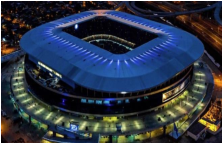
\includegraphics[width=0.69347\linewidth]{figura/screenshot002}
		\label{fig:screenshot002}\\{ Fonte:   http://stadiumdb.com}
	\end{figure}
\end{minipage}\hfill
\begin{minipage}[t!]{0.5\textwidth}
	\begin{itemize}[itemsep=1pt,parsep=1pt]\vspace{0.00mm} 
		\item 	Dados retirados de http://stadiumdb.com \item  Capacidade - 60.540 \item  Construção - 09.2010 -12.2012 \item  Custo - 540 milhões de R\$
	\end{itemize}
\end{minipage} 




\subsection{ALLIANZ PARQUE}
%
\hspace*{1.25 cm} A reconstrução completa de um dos estádios mais bem localizados de São Paulo foi iniciada em 2010, em linha com os preparativos para a Copa do Mundo de 2014. Mas o projeto tinha pouco a ver com o megaevento - era um empreendimento privado do Palmeiras, da WTorre (construtora) e da AEG (maior operadora de entretenimento do mundo). A AEG ganhou acesso ao lucrativo mercado de eventos de São Paulo com este local.\\ 
%
\hspace*{1.25 cm} Desde o início, planejou-se deixar a curva norte da bacia do antigo estádio e incorporá-la ao novo layout. Dessa forma, uma extremidade seria quase retangular, enquanto a outra, oval. O primeiro conceito foi desenhado por Tomas Taveira, enquanto o projeto final ficou a cargo da equipe de Edo Rocha. De acordo com a visão, o revestimento externo consiste em malha metálica perfurada entrelaçada através de estruturas de suporte. O edifício é dominado por cinco torres, que constituem as principais vias de acesso para os torcedores e, ao mesmo tempo, fornecem suporte para a cobertura.\\
\begin{minipage}[t!]{0.5\textwidth}
	\begin{figure}[H]
		\centering  \small 		\caption{Fotografia externa do Estádio Allianz Parque}
		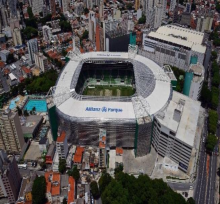
\includegraphics[width=0.69347\linewidth]{figura/screenshot003}
		\label{fig:screenshot003}\\{ Fonte:   http://stadiumdb.com}
	\end{figure}
\end{minipage}\hfill
\begin{minipage}[t!]{0.5\textwidth}
	\begin{itemize}[itemsep=1pt,parsep=1pt]\vspace{0.00mm} 
		\item  Dados retirados de http://stadiumdb.com \item Capacidade - 43.713 \item Construção - 2010 -11/2014 \item Custo - 630 milhões de R\$
	\end{itemize}
\end{minipage} 




\subsection{ESTÁDIO MILTON SANTOS}

\begin{minipage}[t!]{0.5\textwidth}
	\begin{figure}[H]
		\centering  \small 		\caption{Fotografia externa do Estádio Milton Santos}
		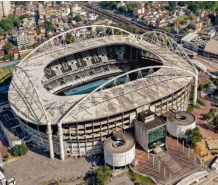
\includegraphics[width=0.6347\linewidth]{figura/screenshot004}
		\label{fig:screenshot004}\\{ Fonte:   http://stadiumdb.com}
	\end{figure}
\end{minipage}\hfill
\begin{minipage}[t!]{0.5\textwidth}
	\begin{itemize}[itemsep=1pt,parsep=1pt]\vspace{0.00mm} 
		\item   Dados retirados de http://stadiumdb.com \item  Capacidade - 44 661 \item  Renovações - 2013, 2016, 2017 \item Custo - 380 milhões de R\$
	\end{itemize}
	
\end{minipage} 




\subsection{ESTÁDIO MARACANÃ}
%
\hspace*{1.25 cm} O Estádio Jornalista Mário Filho, mais conhecido como Maracanã, é um estádio de futebol localizado na Zona Norte da cidade brasileira do Rio de Janeiro. Foi inaugurado em 1950, inicialmente com o nome de Estádio Municipal, durante o mandato do então general de divisão e prefeito do Distrito Federal do Rio de Janeiro Ângelo Mendes de Moraes, tendo sido utilizado na Copa do Mundo de Futebol daquele ano. Quando da sua inauguração, a capacidade oficial de 155 mil lugares fez o Maracanã superar o Hampden Park, de Glasgow, e se tornar o maior estádio do mundo na época.\\ 
%
\hspace*{1.25 cm} Após diversas obras de modernização, a capacidade do estádio é de 78 838 espectadores, sendo o maior estádio do Brasil\\
\begin{minipage}[t!]{0.5\textwidth}
	\begin{figure}[H]
		\centering  \small 	\caption{ Fotografia externa do Estádio Maracanã}
		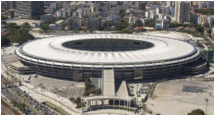
\includegraphics[width=0.69347\linewidth]{figura/screenshot005}
		\label{fig:screenshot005}\\{ Fonte:   http://stadiumdb.com}
	\end{figure}
\end{minipage}\hfill
\begin{minipage}[t!]{0.5\textwidth}
	\begin{itemize}[itemsep=1pt,parsep=1pt]\vspace{0.00mm} 
		\item Dados retirados de http://stadiumdb.com \item Capacidade - 78 838 \item Renovações - 2010-2013 \item Custo -1,14 bilhão de R\$ 
	\end{itemize}	
\end{minipage} 



\subsection{ARENA PANTANAL}
%
\hspace*{1.25 cm} O projeto na zona oeste de Cuiabá foi lançado na primavera de 2010, quando começou a demolição do antigo Verdão. A previsão inicial era de que a obra fosse entregue já em 2012, bem antes da Copa do Mundo de 2014, para a qual o estádio foi encomendado. No entanto, atrasos nas entregas, acidentes e impasses nos pagamentos levaram a atrasos imensos. De fato, o estádio não foi totalmente concluído a tempo para o evento da FIFA de 2014, apesar dos esforços de 1.800 operários no local.\\
\begin{minipage}[t!]{0.5\textwidth}
	\begin{figure}[H]
		\centering  \small 	\caption{ Fotografia externa da Arena Pantanal}
		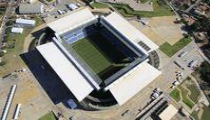
\includegraphics[width=0.69347\linewidth]{figura/screenshot006}
		\label{fig:screenshot006}\\{ Fonte:   http://stadiumdb.com}
	\end{figure}
	
\end{minipage}\hfill
\begin{minipage}[t!]{0.5\textwidth}
	\begin{itemize}[itemsep=1pt,parsep=1pt]\vspace{0.00mm} 
		\item  Dados retirados de http://stadiumdb.com \item Capacidade - 41.930 \item Renovações - 2014 \item Custo - 646 milhões de R\$
	\end{itemize}
	
\end{minipage} 



\subsection{ARENA AMAZONIA}
%
\hspace*{1.25 cm} O estádio está localizado no local do Estádio Vivaldo Lima (comumente chamado de Vivaldão), o antigo maior estádio de Manaus. Embora sua capacidade oficial no fechamento fosse de 31.000 pessoas, o público recorde foi de quase 60.000 pessoas.\\ 
%
\hspace*{1.25 cm} O novo estádio foi batizado de Arena da Amazônia para criar uma referência direta à sua localização e identidade. Seguindo o conceito da GMP Architekten, a estrutura externa do estádio foi projetada para se assemelhar a uma cesta típica da Amazônia, que frequentemente apresenta padrões diagonais. Os assentos do estádio criam um mosaico amarelo-alaranjado que lembra as frutas carregadas na cesta.\\
\begin{minipage}[t!]{0.5\textwidth}
	\begin{figure}[H]
		\centering  \small 		\caption{Fotografia externa da Arena Amazonia}
		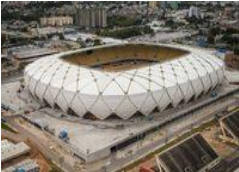
\includegraphics[width=0.69347\linewidth]{figura/screenshot007}
		\label{fig:screenshot007}\\{ Fonte:   http://stadiumdb.com}
	\end{figure}
\end{minipage}\hfill
\begin{minipage}[t!]{0.5\textwidth}
	\begin{itemize}[itemsep=1pt,parsep=1pt]\vspace{0.00mm} 
		\item Dados retirados de http://stadiumdb.com
		\item Capacidade - 44.351
		\item Renovações - 2014
		\item Custo - 669,5 milhões de R\$ 
	\end{itemize}
\end{minipage} 





\subsection{ARENA DAS DUNAS}
%
\hspace*{1.25 cm} As primeiras imagens do estádio foram apresentadas em 2010. Naquela época, a Populous Architects estava no projeto, mas o projeto detalhado foi executado por equipes brasileiras. O estádio, com sua estrutura externa leve e sulcada, tem como característica marcante as escadas expostas, em vez de escondidas sob as arquibancadas.\\
\begin{minipage}[t!]{0.5\textwidth}
	\begin{figure}[H]
		\centering  \small 		\caption{Fotografia externa da Arena das Dunas}
		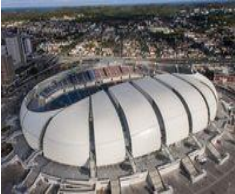
\includegraphics[width=0.69347\linewidth]{figura/screenshot008}
		\label{fig:screenshot008}\\{ Fonte:   http://stadiumdb.com}
	\end{figure}
\end{minipage}\hfill
\begin{minipage}[t!]{0.5\textwidth}
	\begin{itemize}[itemsep=1pt,parsep=1pt]\vspace{0.00mm} 
		\item  Dados retirados de http://stadiumdb.com \item Capacidade - 31.375 \item Inauguração - 2014 \item Custo - 423 milhões de R\$ 
	\end{itemize}
\end{minipage} 





\subsection{ESTÁDIO BEIRA RIO}

%
\hspace*{1.25 cm} A construção do estádio às margens do Rio 1959. As obras foram financiadas por diversas fontes, da torcida do Internacional. Uma das futuras lendas de Porto Alegre foi iniciada em também graças ao engajamento do futebol, Falcão, estava entre os trabalhadores voluntários, então ainda muito jovem.\\
\begin{minipage}[t!]{0.5\textwidth}
	\begin{figure}[H]
		\centering  \small 		\caption{Fotografia externa do Estádio Beira Rio}
		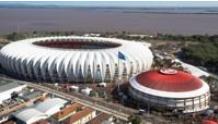
\includegraphics[width=0.69347\linewidth]{figura/screenshot009}
		\label{fig:screenshot009}\\{ Fonte:   http://stadiumdb.com}
	\end{figure}
\end{minipage}\hfill
\begin{minipage}[t!]{0.5\textwidth}
	\begin{itemize}[itemsep=1pt,parsep=1pt]\vspace{0.00mm} 
		\item Dados retirados de http://stadiumdb.com \item Capacidade - 51.800 \item Renovações - 2014 \item Custo - 330 milhões de R\$
	\end{itemize}
	
\end{minipage} 





\subsection{ESTÁDIO PEDRO LUDOVICO TEIXEIRA}
%
\hspace*{1.25 cm} Inicialmente, o estádio estava localizado ao norte do centro, mas, com o tempo, foi se integrando à malha urbana e hoje é o estádio de futebol mais central de Goiânia. Manteve sua forma original até 2006 e foi totalmente demolido posteriormente. A construção do sucessor seria realizada em breve, e a escavação para o novo estacionamento subterrâneo foi feita com antecedência.\\ 
%
\hspace*{1.25 cm} O novo estádio mantém suas funções "olímpicas", oferecendo um campo de jogos e uma pista de atletismo com 8 raias. Com holofotes adicionais, atende à maioria dos critérios nacionais e internacionais. Mesmo após a reconstrução completa, voltou a ser basicamente um estádio de futebol.\\ 
\begin{minipage}[t!]{0.5\textwidth}
	\begin{figure}[H]
		\centering  \small 		\caption{Fotografia externa do Estádio Pedro Ludovico Teixeira}
		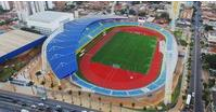
\includegraphics[width=0.69347\linewidth]{figura/screenshot010}
		\label{fig:screenshot010}\\{ Fonte:   http://stadiumdb.com}
	\end{figure}
	
\end{minipage}\hfill
\begin{minipage}[t!]{0.5\textwidth}
	\begin{itemize}[itemsep=1pt,parsep=1pt]\vspace{0.00mm} 
		\item Dados retirados de http://stadiumdb.com \item  Capacidade - 13.500 \item Inauguração - 2016 \item Custo - 96 milhões de R\$ 
	\end{itemize}
\end{minipage} 



\subsection{ESTÁDIO CASTELÃO}
%
\hspace*{1.25 cm} Com o Brasil sendo anunciado como sede da Copa do Mundo de 2014 , outra grande reforma ocorreu em 2011. Desta vez, a arquibancada superior foi mantida, enquanto as arquibancadas inferiores foram reconstruídas, mais próximas do campo e com mais assentos. Apenas a arquibancada principal foi construída completamente do zero, para oferecer instalações para escritórios e serviços de hospitalidade. As obras levaram ao aumento da capacidade, proporcionando também cobertura para todos os espectadores pela primeira vez na história do estádio.\\
\begin{minipage}[t!]{0.5\textwidth}
	\begin{figure}[H]
		\centering  \small 		\caption{Fotografia externa do Estádio Castelão}
		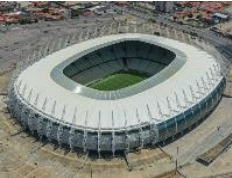
\includegraphics[width=0.69347\linewidth]{figura/screenshot011}
		\label{fig:screenshot011}\\{ Fonte:   http://stadiumdb.com}
	\end{figure}
\end{minipage}\hfill
\begin{minipage}[t!]{0.5\textwidth}
	\begin{itemize}[itemsep=1pt,parsep=1pt]\vspace{0.00mm} 
		\item Dados retirados de http://stadiumdb.com \item Capacidade - 63.903 \item Construção - 2011 / 2013 \item Custo - 518,6 milhões de R\$
	\end{itemize}
	
\end{minipage} 


\subsection{ARENA PERNANBUCO}
%
\hspace*{1.25 cm} As obras nos arredores do Recife começaram em agosto de 2010 e a entrega do novo estádio com muito atraso (nem duas semanas antes da Copa das Confederações de 2013) não é o único resultado do projeto.\\ 
%
\hspace*{1.25 cm} Em maio de 2013, foi assinado um contrato de naming rights de 10 anos com a Itaipava, marca brasileira de cerveja. No valor de cerca de R\$ 100 milhões, o contrato é idêntico ao assinado em Salvador da Bahia e torna o novo estádio pernambucano uma das duas Arenas Itaipava no Brasil.\\
\begin{minipage}[t!]{0.5\textwidth}
	\begin{figure}[H]
		\centering  \small 		\caption{Fotografia externa da Arena Pernambuco}
		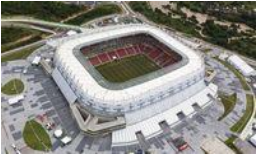
\includegraphics[width=0.69347\linewidth]{figura/screenshot012}
		\label{fig:screenshot012}\\{ Fonte:   http://stadiumdb.com}
	\end{figure}
\end{minipage}\hfill
\begin{minipage}[t!]{0.5\textwidth}
	\begin{itemize}[itemsep=1pt,parsep=1pt]\vspace{0.00mm} 
		\item Dados retirados de http://stadiumdb.com \item Capacidade - 46154 \item Inauguração - 2013 \item Custo - 650 milhões de R\$
	\end{itemize} 
	
\end{minipage} 



\subsection{ARENA MRV}
%
\hspace*{1.25 cm} O projeto para o novo estádio do Atlético Mineiro foi elaborado em 2014, quando o arquiteto Bernardo Farkasvolgyi (torcedor particular do Galo) elaborou o projeto. Um terreno foi adquirido com sucesso da MRV Engenharia, patrocinadora do clube e maior incorporadora do Brasil, com sede em Belo Horizonte, para a construção da arena. Posteriormente, a empresa também adquiriu os direitos de naming do estádio.\\
\begin{minipage}[t!]{0.5\textwidth}
	\begin{figure}[H]
		\centering  \small 	\caption{Fotografia externa da Arena MRV}
		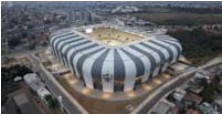
\includegraphics[width=0.69347\linewidth]{figura/screenshot013}
		\label{fig:screenshot013}\\{ Fonte:   http://stadiumdb.com}
	\end{figure}
\end{minipage}\hfill
\begin{minipage}[t!]{0.5\textwidth}
	\begin{itemize}[itemsep=1pt,parsep=1pt]\vspace{0.00mm} 
		\item  Dados retirados de http://stadiumdb.com \item Capacidade - 47.465 \item  Inauguração - 2022 \item Custo - 560 milhões de R\$
	\end{itemize}
\end{minipage} 


%


\subsection{ARENA DO ESPORTE}
%
\hspace*{1.25 cm} Este projeto privado foi alvo de lobby em 2011, mas só tomou forma final com a revelação do projeto da Pontual Arquitetos e Tomas Taveira. O segundo nome deve soar familiar, já que a arena proposta se assemelha a muitos de seus trabalhos anteriores, talvez até demais.\\ 
%
\hspace*{1.25 cm} Sob o revestimento colorido do clube, encontram-se arquibancadas de dois níveis, divididas por três níveis de camarotes comerciais. A capacidade total prevista é de cerca de 46.000 pessoas.\\
\begin{minipage}[t!]{0.5\textwidth}
	\begin{figure}[H]
		\centering  \small 		\caption{Fotografia externa da Arena do Esporte}
		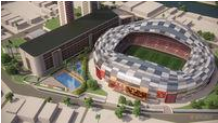
\includegraphics[width=0.69347\linewidth]{figura/screenshot014}
		\label{fig:screenshot014}\\{ Fonte:   http://stadiumdb.com}
	\end{figure}
\end{minipage}\hfill
\begin{minipage}[t!]{0.5\textwidth}
	\begin{itemize}[itemsep=1pt,parsep=1pt]\vspace{0.00mm} 
		\item Dados retirados de http://stadiumdb.com \item Capacidade - 46.000 \item Inauguração - 2016 \item Custo - 600 milhões de R\$
	\end{itemize}
\end{minipage} 




\subsection{ESTÁDIO URBANO CALDEIRA}
%
\hspace*{1.25 cm} Todo o estádio seria envolto em malha de fibra de carbono branca, garantindo ventilação natural. Isso é necessário principalmente porque a cobertura será uma cúpula completa. Em grande parte opaca, a cobertura terá um óculo significativo para fornecer luz natural, com uma tela panorâmica gigante abaixo.\\ 
%
\hspace*{1.25 cm} Atrasos no projeto e custos exorbitantes levaram a mudanças no projeto. Uma das interferências mais visíveis foi o abandono da cobertura total do estádio. Por outro lado, a capacidade das arquibancadas foi aumentada de mais de 25.000 para mais de 30.000 espectadores.\\
\begin{minipage}[t!]{0.5\textwidth}
	\begin{figure}[H]
		\centering  \small 		\caption{Fotografia externa do Estádio Urbano Caldeira}
		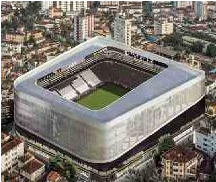
\includegraphics[width=0.69347\linewidth]{figura/screenshot015}
		\label{fig:screenshot015}\\{ Fonte:   http://stadiumdb.com}
	\end{figure}
\end{minipage}\hfill
\begin{minipage}[t!]{0.5\textwidth}
	\begin{itemize}[itemsep=1pt,parsep=1pt]\vspace{0.00mm} 
		\item Dados retirados de http://stadiumdb.com \item Capacidade - 30.108 \item  Inauguração - 2027 \item Custo - 450 milhões de R\$
	\end{itemize}
\end{minipage} 





\subsection{ESTÁDIO INDEPENDÊNCIA}
%
\hspace*{1.25 cm} A demolição do antigo terreno estava planejada para 2008. O América FC recusou o arrendamento do estádio e as obras estavam programadas para começar em 2009. Minas Gerais e o governo federal dividiram o custo entre si, estimado em R\$ 44 milhões. As obras começaram com um atraso de um ano - demolição em janeiro de 2010 e construção de novas arquibancadas em novembro daquele ano. Enormes problemas surgiram ao longo do caminho, com o custo subindo dos primeiros R\$ 44 milhões para 70, 90, 114 e finalmente R\$ 125 milhões.\\
\begin{minipage}[t!]{0.5\textwidth}
	\begin{figure}[H]
		\centering  \small 		\caption{ Fotografia externa do Estádio Independência}
		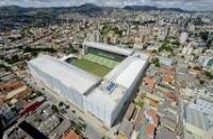
\includegraphics[width=0.69347\linewidth]{figura/screenshot017}
		\label{fig:screenshot017}\\{ Fonte:   http://stadiumdb.com}
	\end{figure}
\end{minipage}\hfill
\begin{minipage}[t!]{0.5\textwidth}
	\begin{itemize}[itemsep=1pt,parsep=1pt]\vspace{0.00mm} 
		\item   Dados retirados de http://stadiumdb.com \item  Capacidade - 23.950 \item Inauguração - 2013 \item Custo - 360 milhões de R\$
	\end{itemize}
\end{minipage} 


\subsection{ARENA DA BAIXADA}
%
\hspace*{1.25 cm} O estádio existente no centro de Curitiba estava programado para ser expandido antes da Copa do Mundo de 2014. Como uma das reformas privadas em todo o Brasil, o objetivo era maximizar os lucros como uma arena multieventos com teto retrátil. No entanto, os painéis móveis foram cortados do plano original devido aos crescentes atrasos.\\ 
%
\hspace*{1.25 cm} O estádio terá um novo lado sul, nova estrutura de cobertura baseada em treliças de aço e uma nova identidade visual.\\
\begin{minipage}[t!]{0.5\textwidth}
	\begin{figure}[H]
		\centering  \small 	\caption{Fotografia externa da Arena da Baixada}
		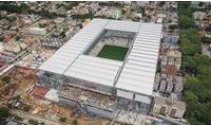
\includegraphics[width=0.69347\linewidth]{figura/screenshot016}
		\label{fig:screenshot016}\\{ Fonte:   http://stadiumdb.com}
	\end{figure}
\end{minipage}\hfill
\begin{minipage}[t!]{0.5\textwidth}
	\begin{itemize}[itemsep=1pt,parsep=1pt]\vspace{0.00mm} 
		\item Dados retirados de http://stadiumdb.com \item Capacidade - 41.375 \item Inauguração - 2012 \item Custo - 360 milhões de R\$
	\end{itemize}
\end{minipage} 


% ------
%!TEX root = ..//Avali-Arena-Esportivas.tex
\section{METODOLOGIA}
%
\hspace*{1.25 cm} Em função das características do imóvel avaliando, do mercado imobiliário e da pesquisa realizada adotou-se o Método Evolutivo \(Vi = (Vt + Cb) * FC \) , por ser o que melhor reflete a realidade do imóvel avaliando.\\ 
%
\hspace*{1.25 cm} Diz a Norma: “8.2.4 - A composição do valor total do imóvel avaliando pode ser obtida através da conjugação de métodos, a partir do valor do terreno, considerados o custo de reprodução das benfeitorias devidamente depreciado e o fator de comercialização”,\\ 
%
\hspace*{1.25 cm} No presente caso, tanto o valor do terreno, e o custo das benfeitorias, foram obtidos pelo Método Comparativo Direto de Dados de Mercado - MCDDM.
% ------
%!TEX root = ..//Avali-Arena-Esportivas.tex

\section{ANÁLISE DO TRATAMENTO ESTATÍSTICO - CUSTO BENFEITORIAS / TERRENO}

\subsection{AMOSTRA ESTÁDIO - CUSTO BENFEITORIAS}
%
\hspace*{1.25 cm} Para o tratamento estatístico (tratamento científico com modelos de regressão linear) no cálculo do valor da construção, foi realizado com o software SisDEA. A amostra utilizada é composta de 16 (dezesseis) dados efetivamente usados, descritos.\\ 
%
\hspace*{1.25 cm} Convém ressaltar que foram adotadas, além da variável dependente, 3 (três) variáveis independentes.\\ 
%
\hspace*{1.25 cm} Conforme já mencionado, foram adotadas, no tratamento estatístico científico, quatro variáveis independentes, ou explicativas, as quais são descritas a seguir:
\begin{description}[itemsep=1pt,parsep=1pt]\vspace{0.00mm} 
	\item[DT (data)]  : variável quantitativa aplicada para indicar a data (ano) de inauguração de cada estádio pesquisado.
	\item[T1 (Padrão 1)]  : Variável dummy, ou dicotômica, aplicada para indicar Código 1 = Arena que possui vários espaços multiusos como: área para treinamentos, convenções, lançamento de produtos, formaturas, festas infantis, restaurantes barbearia, lounge temáticos, halls, camarotes diversos, coworking, shows e inovações tecnológicas como reconhecimento facial, telões de LED, controle de acesso.
	\item[T2 (Padrão 2)]  : Variável dummy, ou dicotômica, Código 0 = Arena que possui alguns espaços multiusos dentre os contemplados no código 1.
	\item[R\$/ASSENTO]  : Variável dependente, ou variável a ser explicada, representa o custo de construção de cada estádio por número de lugares (assentos), ou seja, o custo total de construção, dividido pelo número total de assentos. 
\end{description}
%
\begin{table}[h!t]
	\centering
	\begin{threeparttable}
		\caption{Atributos de Entrada do Terreno Avaliado }
		\label{Tabela-variaveis}
		\begin{tabular}{p{13cm}lp{5cm} l}
			\toprule
			Variável & Atributo    	 \\\midrule
			N de Assentos	& 50.000,00 	 \\	 
			Tipo de Arena	& 0 \\	 
			Data de Inauguração	&12      \\\bottomrule
		\end{tabular}%
		\begin{tablenotes}
			\item [{\normalsize Fonte:     Elaborado pelos Autores (2025)}]  
		\end{tablenotes}
	\end{threeparttable}
\end{table}
\hspace*{1.25 cm} Em relação às duas variáveis dicotômicas, é importante destacar que foram identificados, na amostra, três padrões distintos de estádios esportivos. As duas variáveis dicotômicas adotadas foram suficientes para explicar as diferenças entre os padrões existentes, uma vez que, se P1 e P2 assumirem a posição “não”, resta então o terceiro padrão identificado, referente à estádios esportivos com estrutura tecnológica básica, não preparados para múltiplos usos.
%
%

\begin{longtable}[c]{p{1cm}lp{4cm}l l l lp{3cm}l}
	\caption{Amostra do Tratamento Estatístico da construção.}\\ \toprule
	Item & Endereço & Informante & T1 & T2 &Data &R\$ / Assento    \\ 
	\endfirsthead
	\multicolumn{6}{c} {{\tablename\ \thetable{} -- Contin\'ua na p\'agina anterior}} \\    \toprule
	Item & Endereço & Informante & T1 & T2 &Data &R\$ / Assento    \\  \midrule
	\endhead
	\midrule
	%	\multicolumn{6}{r}{{Contin\'ua na pagina seguinte...}}\\ \midrule
	\endfoot
	\bottomrule
	%Item & Endereço & Informante & T1 & T2 &Data &R\$ / Assento    	 \\
	1&	Grêmio	&http	"stadiumdb.com	&0	&0	&3	&8.919,72\\ 
	2&	Allianz Parque	&http	"stadiumdb.com	&1&	0	&3&	14.412,19\\ 
	3&	Engenhão&	http	"stadiumdb.com	&0&	0&	6	&8.508,54\\ 
	4&	Maracanã&	http	"stadiumdb.com	&1&	0&	2&	14.460,03\\ 
	5&	Arena Pantanal&	http	//stadiumdb.com	&1	&0&	3	&15.607,63\\ 
	6&	Amazônia&	http	//stadiumdb.com	&1&	0&	3&	15.095,49\\ 
	7&	Arena das Dunas	&http	//stadiumdb.com	 &1	&0&	3	&13.482,07\\ 
	8&	Beira-Rio&	http	//stadiumdb.com&	0&	0&	3	&6.370,66\\ 
	9&	Estádio Pedro &http	//stadiumdb.com&	0&	0&	5	&7.111,11\\ 
	10&	Novo Castelão&	http	//stadiumdb.com	&0&1	&2	&8.115,42\\ 
	11	&Arena Pernambuco&	http	//stadiumdb.com& 1&	0&	2	&14.083,29\\  
	12&	Arena MRV &http	//stadiumdb.com&	0&	1&	11	&11.798,17\\ 
	13&Arena do Esporte&http	//stadiumdb.com	&0	&1	&5	&13.043,48\\ 
	14	&Urbano Caldeira&	http	//stadiumdb.com&0&	1&	14	&14.946,13\\  
	15&Independência&http	//stadiumdb.com	&0	&0	&1	&5.212,21\\ 
	16&Arena da Baixada&http	//stadiumdb.com&0&0&2&8.700,91\\  
\end{longtable}
Fonte:     Elaborado pelos Autores (2025)

\subsection{MODELO ESTATÍSTICO DO TRATAMENTO CIENTÍFICO - SisDEA}
\begin{table}[h!t]
	\centering
	\begin{threeparttable}
		\caption{Atributos de Entrada do Terreno Avaliado }
		\label{Tabela-variavedis}
		\begin{tabular}{lll}
			\toprule
			\multicolumn{3}{l}{Modelo do SisDea}                   \\\midrule
			Modelo                & XXX               &             \\
			Data da criação       & 16/02/025         &             \\
			Área de concentração  & Avaliação de Bens &             \\
			Tipologia em estudo   & Outras            &             \\
			Dados do Modelo       & 16                &             \\
			Dados utilizados      & 4                 &             \\
			Variáveis utilizadas  & 4                 &             \\
			& Regressão         & Estimativa  \\
			Coef. de correlação   & 0,937227481       & 0,945805744 \\
			Coef. de determinação & 0,878395351       & 0,894548505 \\
			Desvio Padrão         & 0,138222614       & 1295,022687 \\
			&                   &             \\
			Normalidade:          & \multicolumn{2}{c}{68,93,100}    \\\bottomrule
		\end{tabular}
		\begin{tablenotes}
			\item [{\normalsize Fonte:     Elaborado pelos Autores (2025)}]  
		\end{tablenotes}
	\end{threeparttable}
\end{table}

\begin{comment}
	| Modelo do SisDEA |		\\ 
	Modelo:	XXXXXXX	\\ 
	Data de criação:	16/02/2025	\\ 
	Área de concentração:	Avaliação de Bens	\\ 
	Tipologia em estudo:	Outras	\\ 
	Dados do modelo:	16	\\ 
	Dados utilizados:	16	\\ 
	Variáveis do modelo:	4	\\ 
	Variáveis utilizadas:	4	\\ 
	\\ 
	Regressão	Estimativa\\ 
	Coef. de correlação	0,937227481	0,945805744\\ 
	Coef. de determinação	0,878395351	0,894548505\\ 
	Desvio padrão	0,138222614	1295,022687\\ 	 
\end{comment}

\subsubsection{RESULTADOS}

\begin{minipage}[t!]{0.5\textwidth}
	\begin{figure}[H]
		\centering  \small 		\caption{ Resultados pelo SISDEA}
		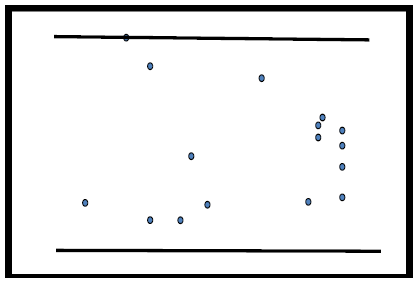
\includegraphics[width=0.9347\linewidth]{figura/screenshot030}
		\label{fig:screenshot030}
	\end{figure}
	
\end{minipage}\hfill
\begin{minipage}[t!]{0.5\textwidth}
	\begin{figure}[H]
		\centering  \small 		\caption{ Resultados pelo SISDEA}
		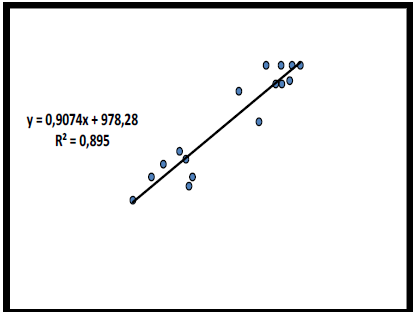
\includegraphics[width=0.9347\linewidth]{figura/screenshot031}
		\label{fig:screenshot031}
	\end{figure}
\end{minipage} 
\begin{center}
	Fonte: Elaborado pelos Autores, pelo SISDEA
\end{center}

\begin{figure}[H]
	\centering  \small 		\caption{ Resultados pelo SISDEA}
	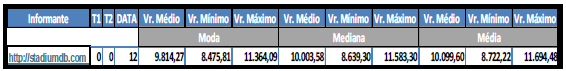
\includegraphics[width=0.947\linewidth]{figura/screenshot032}
	\label{fig:screenshot032}\\{ Fonte: Elaborado pelos Autores, pelo SISDEA}
\end{figure}


\begin{comment}
	%
	\hspace*{1.25 cm} Caracterização do im óvel avaliando	Completa quanto a todas as variáveis analisadas	Completa quanto às Adoção de situação variáveis utilizadas no modelo paradigma	3\\ 
	%
	\hspace*{1.25 cm} Quantidade mínima de dados de mercado, efetivamente utilizados	6 (k+1), onde k é o número de variáveis independentes	4 (k+1), onde k é o 3 (k+1), onde k é o número de variáveis número de variáveis independentes independentes	2\\ 
	%
	\hspace*{1.25 cm} Identificação dos dados de Imdeenrctaifdicoação dos dados de	Apresentação de informações relativas a todos os dados e variáveis analisados na modelagem, com foto e características observadas pelo autor do laudo	Apresentação de Apresentação de informações relativas a informações relativas todos os dados e aos dados e variáveis variáveis analisados na efetivamente utilizados modelagem no modelo	3\\ 
	—	Não admitida	Admitida, desde que: Admitida para apenas a) as medidas das uma variável, desde características do imóvel que: a) as medidas das avaliando não sejam características do imóvel superiores a avaliando não sejam 100 \% do limite superiores a 100\% do amostral superior, nem nem inferiores à limite amostral inferior metade do limite b) o valor estimado não amostral inferior, b) o ultrapasse 20 \% do valor valor estimado não calculado no limite da ultrapasse 15\% do valor fronteira amostral, para calculado no limite da as referidas variáveis, de fronteira amostral, para per si e a referida variável simultaneamente, e em módulo	3\\ 
	Nível de significância (som atório do valor das duas caudas) máximo para a rejeição da hipótese nula de cada regressor (teste bicaudal)	10\%	20\% 30\%	3\\ 
	Nível de significância máximo admitido para a rejeição da hipótese nula do modelo através do teste F de Snedecor	1\%	2\% 5\%	\\ 
	10 6	17\\ 
	2, 4, 5 e 6 no grau III e os demais no mínimo no	2, 4, 5 e 6 no mínimo no  , ,. Todos, no mínimo no grau II e os dem ais no grau I mínimo no grau I	\\ 
	Grau de Fundamentação do Laudo				 
\end{comment}

\begin{figure}[H]
	\centering  \small 		\caption{ Resultados pelo SISDEA}
	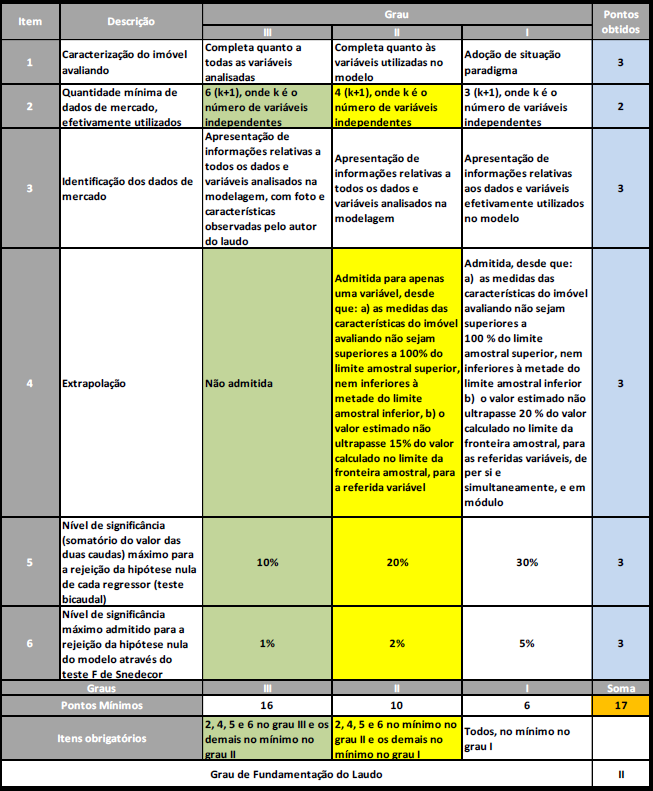
\includegraphics[width=0.947\linewidth]{figura/screenshot033}
	\label{fig:screenshot033}\\{ Fonte: Elaborado pelos Autores, pelo SISDEA}
\end{figure}

\subsection{AMOSTRA ESTÁDIO VALOR DO TERRENO}
%
\hspace*{1.25 cm} Para o tratamento estatístico (tratamento científico com modelos de regressão linear) no cálculo do valor da construção, foi realizado com o software SisDEA. A amostra utilizada é composta de 46 (quarenta e seis) dados efetivamente usados, descritos no item 2 deste trabalho.\\ 
%
\hspace*{1.25 cm}  Convém ressaltar que foram adotadas, além da variável dependente, 4 (quatro) variáveis independentes.\\ 
%
\hspace*{1.25 cm}  Conforme já mencionado, foram adotadas, no tratamento estatístico científico, quatro variáveis independentes, ou explicativas, as quais são descritas a seguir:
%
\begin{description}[itemsep=1pt,parsep=1pt]\vspace{0.00mm} 
	\item[\textbf{Valor / m2}]   - Variável dependente ou explicada. Valor que queremos calcular. Identifica o valor total dividido pela área total do imóvel.
	
	\item[\textbf{Área total}]   - Variável independente quantitativa das áreas totais dos terrenos pesquisados. A hipótese formulada busca mostrar que quanto maior a área menor o valor unitário, tendo em vista as leis de mercado.
	
	\item[\textbf{Indice fiscal (PMS)}]   - Variável independente proxy que indica a proporção do Índice Fiscal da Prefeitura Municipal do Salvador dos imóveis pesquisados. A hipótese formulada busca mostrar que quanto maior a atratividade maior o valor unitário.
	
	\item[\textbf{Vocação} ]  - Variável independente qualitativa representada por códigos alocados, que indica a vocação dos imóveis pesquisados, sendo: 1 = Residencial Unifamiliar; 2 = Residencial Multifamiliar e 3 = Comercial.
	
	\item[\textbf{CAB PDDU}]   - Variável independente proxy que indica o CAB dos imóveis pesquisados. A hipótese formulada busca mostrar que quanto maior a atratividade maior o valor unitário
\end{description}


\begin{table}[ht]
	\centering
	\begin{threeparttable}
		\caption{Atributos de Entrada do Terreno Avaliado }
		\label{Tabela-entrada-avaliado}
		\begin{tabular}{p{13.0cm}l  l}
			\toprule
			Variavel & Atributo    	 \\\midrule
			Area total	& 129.277,00 	 \\	 
			Setor Urbano	& 45,07 \\	 
			Vocacao	&3     \\	 
			CAB	& 1,05    \\\bottomrule
		\end{tabular}%
		\begin{tablenotes}
			\item [{\normalsize Fonte:     Elaborado pelos Autores (2025)}]  
		\end{tablenotes}
	\end{threeparttable}
\end{table}

\subsection{MODELO ESTATÍSTICO DO TRATAMENTO CIENTÍFICO - SisDEA}

\begin{table}[h!t]
	\centering
	\begin{threeparttable}
		\caption{Resultado do Terreno Avaliado }
		\label{Tabela-entrada-avalia5do}
		\begin{tabular}{p{2.5cm}lp{1.0cm}lp{2.5cm}lp{1.0cm}lp{1.5cm}lp{2.0cm}lp{1.0cm}lp{1.0cm}ll}
			\toprule
			Variável&	Média&	Mínimo&	Máximo&	Coeficiente&	t&	Sig(\%)	&transf 	 \\\midrule
			Área total&	86,34&	18,97&	367,42&	0,00&	4,84&	0,00&	th\\ 
			Índice Fiscal (PMS)&	0,03&	0,01&	0,08&	0,25&	8,11	&0,00&	1/x\\ 
			Vocação	&2,33&	1,00&	3,00&	0,00&	-6,22&	0,00&	x\\ 
			CAB (PDDU)	&1,38&	0,50&	2,00&	-0,01&	-11,04&	0,00&	x\\ 
			Valor Unitário	&0,03&	0,01&	0,04&	0,04&	20,31&	0,00	&1/yh \\\bottomrule
		\end{tabular}%
		\begin{tablenotes}
			\item [{\normalsize Fonte:     Elaborado pelos Autores (2025)}]  
		\end{tablenotes}
	\end{threeparttable}
\end{table}

\begin{table}[h!t]
	\centering
	\begin{threeparttable}
		\caption{Resultado do Terreno Avaliado }
		\label{Tabela-entrada-avaliafd5do}
		\begin{tabular}{p{3.0cm}lp{1.0cm}lp{2.0cm}lp{2.0cm}lp{1.5cm}l}
			\toprule
			\multicolumn{5}{c}{Análise da Variância} 	\\ \midrule
			Fonte de Variação &Soma  dos Quadrados &Graus de Liberdade& Quadrado Médio &F \par calculado\\  \midrule
			Explicada	&0,001535576&	4&	0,00038389&57,09	\\ 
			Não \par  explicada & 0,00027568	&41	&6,72 E-06	& 	\\ 
			Total&	0,001811257	&45	 & & & \\\bottomrule
		\end{tabular}%
		\begin{tablenotes}
			\item [{\normalsize Fonte:     Elaborado pelos Autores (2025)}]  
		\end{tablenotes}
	\end{threeparttable}
\end{table}



\begin{minipage}[t!]{0.5\textwidth}
	\begin{figure}[H]
		\centering  \small 		\caption{ Resultados pelo SISDEA}
		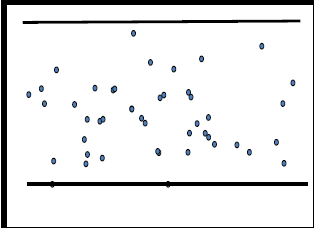
\includegraphics[width=0.93947\linewidth]{figura/screenshot036}
		\label{fig:screenshot036}
	\end{figure}
\end{minipage}\hfill
\begin{minipage}[t!]{0.5\textwidth}
	\begin{figure}[H]
		\centering  \small 		\caption{ Resultados pelo SISDEA}
		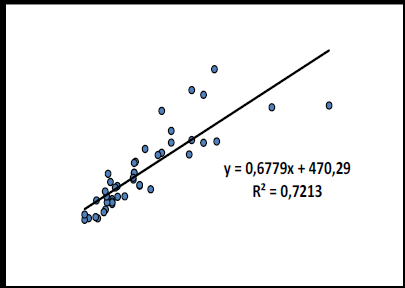
\includegraphics[width=0.93947\linewidth]{figura/screenshot035}
		\label{fig:screenshot035}
	\end{figure}
\end{minipage} 
\begin{center}
	Fonte: Elaborado pelos Autores, pelo SISDEA
\end{center}





\subsubsection{ESTIMATIVAS}

\begin{table}[ht]
	\centering
	\begin{threeparttable}
		\caption{Amostra do Tratamento Estatístico do Custo das Benfeitorias }
		\label{Tabela-e1}
		\begin{tabular}{lp{2.0cm} lp{2.5cm} l p{1.0cm}l p{2.5cm}lp{2.0cm} lp{1.5cm} l}
			\toprule
			Area total &	Índ. Fiscal (PMS)	&Vocação &CAB (PDDU)&	Vr. Médio&	Vr. Mínimo&	Vr. Máximo\\\midrule
			129.277,00&	45,07&	3&	1,5	&1.126,96&	985,20&	1.301,67\\ \bottomrule
		\end{tabular}%
		\begin{tablenotes}
			\item [{\normalsize Fonte:     Elaborado pelos Autores (2025)}]  
		\end{tablenotes}
	\end{threeparttable}
\end{table}
\begin{comment}
	
	
\end{comment}
\begin{figure}[H]
	\centering  \small 		\caption{ Amostra do Tratamento Estatístico do terreno}
	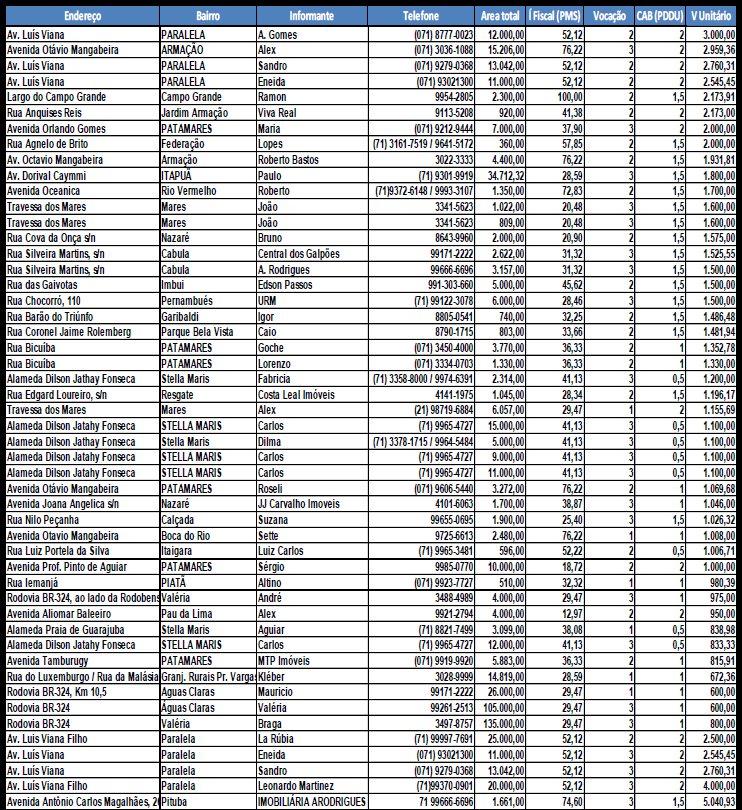
\includegraphics[width=0.947\linewidth]{figura/screenshot037}
	\label{fig:screenshot037}\\{ Fonte: Elaborado pelos Autores, pelo SISDEA}
\end{figure}

\begin{comment}
	\newpage
	\begin{landscape}
		\begin{longtable}[c]{p{2cm}p{1.5cm}lp{1.0cm}lp{0.5cm}lp{0.5cm}lp{0.5cm}lp{0.5cm}lp{0.5cm}lp{0.5cm}lp{0.5cm}l}
			\caption{Tabla de varias p\'aginas con encabezado y pie.}\\ \toprule
			Endereço	&Bairro&	Informante	&Telefone&	Área total& Fiscal \par (PMS)&Vocação&(PDDU)& V Unitário \\ \midrule
			\endfirsthead
			\multicolumn{9}{c} {{\tablename\ \thetable{} -- continua de la p\'agina		anterior}} \\    \toprule
			Endereço	&Bairro&	Informante	&Telefone&	Área total& Fiscal \par (PMS)&Vocação&(PDDU)& V Unitário \\ \midrule
			\endhead
			\midrule
			\multicolumn{9}{r}{{Contin\'ua en la siguiente p\'agina...}}\\ \midrule
			\endfoot
			\bottomrule
			%\endlasthead
			%Endereço	&Bairro&	Informante	&Telefone&	Área total& Fiscal \par (PMS)&Vocação&(PDDU)& V Unitário	 \\\midrule
			Av. Luís Viana&	Paralela&	A. Gomes&	(071) 8777-0023	&12.000,00&52,12&	2&	2&	3.000,00\\ 
			Avenida Otávio Mangabeira&	ARMAÇAO	Alex&	(071) 3036-1088&	15.206,00&	76,22	&3	&2	&2.959,36\\ 
			Av. Luís Viana	&PARALELA	Sandro&	(071) 9279-0368	&13.042,00&	52,12&	2	&2	&2.760,31\\ 
			Av. Luís Viana	&PARALELA	Eneida	&071) 93021300	&11.000,00	&52,12&	2&	2&	2.545,45\\ 
			Largo do Campo Grande	&Campo Grande	Ramon&	9954-2805&	2.300,00&	100,00	&2&	1,5	2.173,91\\ 
			Rua Anquises Reis&	Jardim Armação	Viva Real&	9113-5208&	920,00&	41,38&	2&	2&	2.173,00\\ 
			Avenida Orlando Gomes	&PATAMARES	Maria&	(071) 9212-9444	&7.000,00v	37,90	&3	2&	2.000,00\\ 
			Rua Agnelo de Brito	&Federação	Lopes	&(71) 3161-7519 / 9641-5172	&360,00	&57,85&	2&	1,5	&2.000,00\\ 
			Av. Octavio Mangabeira	&Armação&	Roberto Bastos&	3022-3333	&4.400,00	&76,22&	2&	1,5	1.931,81\\ 
			Av. Dorival Caymmi	&ITAPUA	Paulo&	(71) 9301-9919	&34.712,32&	28,59&	3&	1,5	&1.800,00\\ 
			Avenida Oceanica&	Rio Vermelho&	Roberto	&(71)9372-6148 / 9993-3107&	1.350,00&	72,83&	2&	1,5&	1.700,00\\ 
			Travessa dos Mares	&Mares	João&	3341-5623&	1.022,00&	20,48 	3&	1,5	&1.600,00\\ 
			Travessa dos Mares	&Mares	João&	3341-5623	&809,00&	20,48	&3&	1,5	&1.600,00\\ 
			Rua Cova da Onça s/n&	Nazaré	Bruno&	8643-9960&	2.000,00&	20,90&	2&	1,5&	1.575,00\\ 
			Rua Silveira Martins, s/n	&Cabula	Central dos Galpões	&99171-2222	&2.622,00&	31,32	3	&1,5&	1.525,55\\ 
			Rua Silveira Martins, s/n&	Cabula&	A. Rodrigues&	99666-6696&	3.157,00&	31,32&	3&	1,5&	1.500,00\\ 
			Rua das Gaivotas&	Imbui	&Edson Passos&	991-303-660	&5.000,00&	45,62	2&	1,5	&1.500,00\\ 
			Rua Chocorró, 110	&Pernambués	URM	&(71) 99122-3078	&6.000,00&	28,46	&3	&1,5&	1.500,00\\ 
			Rua Barão do Triúnfo&	Garibaldi&	Igor	&8805-0541&	740,00	&32,25	2	&1,5	&1.486,48\\ 
			Rua Coronel Jaime Rolemberg	&Parque Bela Vista	&Caio	&8790-1715&	803,00	&33,66&	2&	1,5	&1.481,94\\ 
			Rua Bicuíba	PATAMARES&	Goche&	(071) 34504000&	3.770,00&	36,33&	2&	1	&1.352,78\\ 
			Rua Bicuíba	PATAMARES&	Lorenzo&	(071) 3334-0703	&1.330,00&	36,33	&2	&1&	1.330,00\\ 
			Alameda Dilson Jathay Fonseca&	Stella Maris	&Fabricia&	(71) 3358-8000 / 9974-6391	&2.314,00&	41,13	3&	0,5	&1.200,00\\ 
			Rua Edgard Loureiro, s/n	&Resgate&	Costa Leal Imóveis	&4141-1975&1.045,00	28,34&	2	&1,5&	1.196,17\\ 
			Travessa dos Mares	Mares&	Alex &	(21) 98719-6884	&6.057,00	&29,47&	1&	2	&1.155,69\\ 
			Alameda Dilson Jatahy Fonseca&	STELLA MARIS&	Carlos	(71) 99654727&	15.000,00&	41,13&	3&	0,5	&1.100,00\\ 
			Alameda Dilson Jathay Fonseca	&Stella Maris&	Dilma&	(71) 3378-1715 / 9964-5484&	5.000,00&	41,13&	3&	0,5	&1.100,00\\ 
			Alameda Dilson Jatahy Fonseca&	STELLA MARIS&	Carlos	(71) 99654727&	9.000,00&	41,13	&3	&0,5&	1.100,00\\ 
			Alameda Dilson Jatahy Fonseca&	STELLA MARIS&	Carlos&	(71) 99654727	&11.000,00&	41,13&	3&	0,5&	1.100,00\\ 
			Avenida Otávio Mangabeira	&PATAMARES&	Roseli	&(071) 9606-5440&	3.272,00&	76,22	&2	&1	&1.069,68\\ 
			Avenida Joana Angelica s/n	&Nazaré	JJ Carvalho Imoveis 	4101-6063	&1.700,00&	38,87&	3&	1&	1.046,00\\ 
			Rua Nilo Peçanha&	Calçada	Suzana	99655-0695	&1.900,00&	25,40&	3	&1,5&	1.026,32\\ 
			Avenida Otavio Mangabeira&	Boca do Rio	Settev	9725-6613&	2.480,00&	76,22&	1&	1&	1.008,00\\ 
			Rua Luiz Portela da Silva&	Itaigara	Luiz Carlos&	(71) 9965-3481&	596,00	&52,22	&2&	0,5	&1.006,71\\ 
			Avenida Prof. Pinto de Aguiar&	PATAMARES&	Sérgio&	9985-0770	&10.000,00&	18,72	&2&	2&	1.000,00\\ 
			Rua Iemanjá	PIATA	&Altino	(071) 9923-7727	&510,00	&32,32&	1&	1	&980,39\\ 
			Rodovia BR-324, ao lado da Rodobens	&Valéria	&André	&34884989&	4.000,00	&29,47&	3&	1	&975,00\\ 
			Avenida Aliomar Baleeiro&	Pau da Lima	&Alex	9921-2794&	4.000,00&	12,97	&2	&2	&950,00\\ 
			Alameda Praia de Guarajuba	&Stella Maris&	Aguiar&	(71) 8821-7499	3&.099,00	&38,08&	1&	0,5	&838,98\\ 
			Alameda Dilson Jatahy Fonseca	&STELLA MARIS&	Carlos	(71) 99654727&	12.000,00&	41,13&	3&	0,5&	833,33\\ 
			Avenida Tamburugy	&PATAMARES	MTP Imóveis	&(071) 9919-9920	5.883,00	&36,33&	2&	1	&815,91\\ 
			Rua do Luxemburgo / Rua da Malásia	&Grani. Rurais Pr. Varga&	Kléber	3028-9999	&14.819,00	&28,59	&1&	1	&672,36\\ 
			Rodovia BR-324, Km 10,5	&Aguas &Claras	Mauricio	&99171-2222	&26.000,00&	29,47&	1&	1&	600,00\\ 
			Rodovia BR-324&	Águas Claras&	Valéria	99261-2513	&105.000,00	&29,47v	3	&1&	600,00\\ 
			Rodovia BR-324&	Valéria	Braga&	3497-8757&	135.000,00	&29,47&	3	&1	&800,00\\ 
			Av. Luis Viana Filho	&Paralela&	La Rúbia&	(71) 99997-7691	&25.000,00	&52,12	2&	2&	2.500,00\\ 
			Av. Luís Viana	&Paralela	Eneid&a	(071) 93021300&	11.000,00&	52,12&	3&	2&	2.545,45\\ 
			Av. Luís Viana	&Paralela	Sandro&	(071) 9279-0368&	13.042,00&	52,12&	3&	2	&2.760,31\\ 
			Av. Luís Viana &Filho	Paralela&	Leonardo Martinez&	(71) 99370 - 0901&	20.000,00&	52,12	&3&	2&	4.000,00\\ 
			Avenida Antônio Carlos Magalhães, 2	&Pituba&	IMOBILIÁRIA ARODRIGUES	&71 99666 - 6696&	1.661,00&	74,60&	3	&1,5&	5.040,93 \\ 
		\end{longtable}
	\end{landscape} 	 
\end{comment}

\begin{figure}[H]
	\centering  \small 		\caption{ Amostra do Tratamento Estatístico do terreno}
	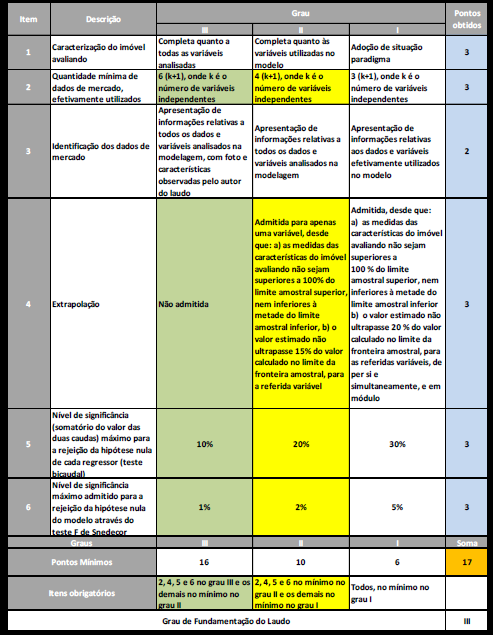
\includegraphics[width=0.947\linewidth]{figura/screenshot038}
	\label{fig:screenshot038}\\{ Fonte: Elaborado pelos Autores, pelo SISDEA}
\end{figure}
\begin{comment}
	FUNDAMENTAÇÃO\\ 
	Item Descrição		III	Grau	I	Pontos obtidos\\ 
	1	Caracterização do imóvel avaliando	Completa quanto a todas as variáveis analisadas	Completa quanto às variáveis utilizadas no modelo	Adoção de situação paradigma	3\\ 
	2	Quantidade mínima de dados de mercado, efetivamente utilizados	6 (k+1), onde k é o número de variáveis independentes	4 (k+1), onde k é o número de variáveis independentes	3 (k+1), onde k é o número de variáveis independentes	3\\ 
	Identificação dos dados de mercado	Apresentação de informações relativas a todos os dados e variáveis analisados na modelagem, com foto e características observadas pelo autor do laudo	Apresentação de informações relativas a todos os dados e variáveis analisados na modelagem	Apresentação de informações relativas aos dados e variáveis efetivamente utilizados no modelo	2\\ 
	4	Extrapolação	Não admitida	Admitida para apenas uma variável, desde que: a) as medidas das características do imóvel avaliando não sejam superiores a 100\% do limite amostral superior, nem inferiores à metade do limite amostral inferior, b) o valor estimado não ultrapasse 15\% do valor calculado no limite da fronteira amostral, para a referida variável	Admitida, desde que: a)	as medidas das características do imóvel avaliando não sejam superiores a 100 \% do limite amostral superior, nem inferiores à metade do limite amostral inferior b)	o valor estimado não ultrapasse 20 \% do valor calculado no limite da fronteira amostral, para as referidas variáveis, de per si e simultaneamente, e em módulo	3\\ 
	Nível de significância (somatório do valor das duas caudas) máximo para a rejeição da hipótese nula de cada regressor (teste bicaudal)	10\%	20\%	30\%	3\\ 
	6	Nível de significância máximo admitido para a rejeição da hipótese nula do modelo através do teste F de Snedecor	1\%	2\%	5\%	3\\ 
	Graus III				Soma\\ 
	Pontos Mínimos	16	10	6	17\\ 
	I	tens obrigatórios	2, 4, 5 e 6 no	  grau III e os demais no mínimo no grau II	2, 4, 5 e 6 no mínimo no grau II e os demais no mínimo no grau I	Todos, no mínimo no grau I	\\ 
	Grau de Fundamentação do Laudo		
\end{comment}

% ------
%!TEX root = ..//Avali-Arena-Esportivas.tex
\section{MÉTODO EVOLUTIVO}
\subsection{DETERMINAÇÃO DO VALOR TOTAL DA ARENA}
\begin{equation}
	Metodologia - Valor \, Total \, do \, Imovel - Metodo \, Evolutivo
\end{equation}

%
\hspace*{1.25 cm} Em função das características do imóvel avaliando, do mercado imobiliário local e da pesquisa realizada adotou-se o método acima por ser o que melhor reflete a realidade do imóvel avaliando.\\ 
%
\hspace*{1.25 cm} Diz a Norma: “\textit{8.2.4 - A composição do valor total do imóvel avaliando pode ser obtida através da conjugação de métodos, a partir do valor do terreno, considerados o custo de reprodução das benfeitorias devidamente depreciado e o fator de comercialização}”, ou seja:\\

\begin{minipage}[t!]{0.35\textwidth}
	\begin{equation}
		VI = (VT + CB) x FC  
	\end{equation}		
	
\end{minipage}\hfill
\begin{minipage}[t!]{0.5\textwidth}
	Onde:\\ 
	VI =	Valor do imóvel\\ 
	VT =	Valor do terreno\\ 
	CB =	Custo de reedição da benfeitoria\\ 
	FC =	Fator de comercialização\\ 
\end{minipage} 


\begin{figure}[H]
	\centering  \small 		\caption{ Amostra do Tratamento Estatístico do terreno}
	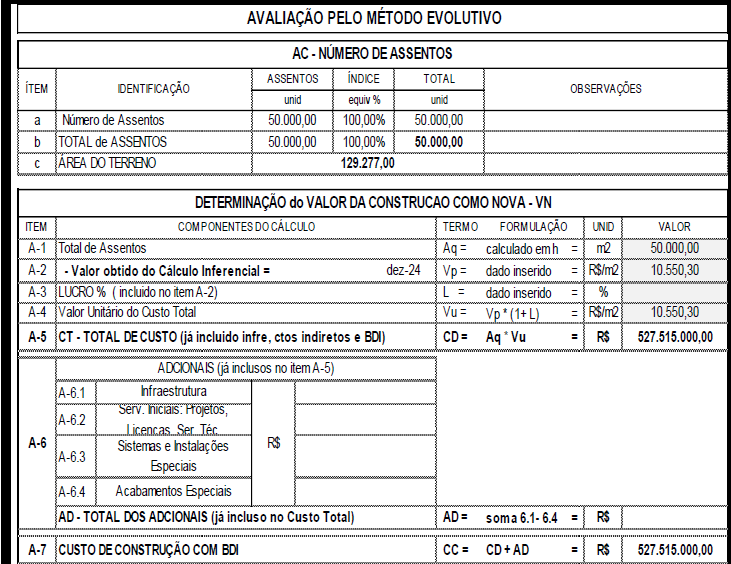
\includegraphics[width=0.94947\linewidth]{figura/screenshot039}
	\label{fig:screenshot039}\\{ Fonte: Elaborado pelos Autores }
\end{figure}

\begin{figure}[H]
	\centering  \small 		\caption{ Amostra do Tratamento Estatístico do terreno}
	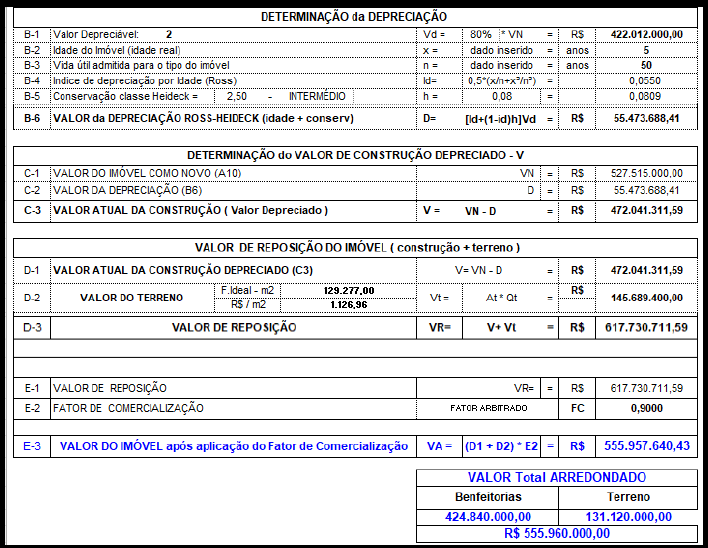
\includegraphics[width=0.94947\linewidth]{figura/screenshot040}
	\label{fig:screenshot040}\\{ Fonte: Elaborado pelos Autores }
\end{figure}

\begin{comment}
	AVALIAÇÃO PELO MÉTODO EVOLUTIVO					\\ 
	AC - NÚMERO DE ASSBNTOS					\\ 
	ÍTEM	IDENTIFICAÇÃO	ASSENTOS	INDICE	TOTAL	OBSERVAÇÕES\\ 
	unid	equiv \%	unid	\\ 
	Número de Assentos	50.000,00	100,00\%	50.000,00 :	\\ 
	TOTAL de ASSENTOS	50.000,00	100,00\%	50.000,00 ?	\\ 
	ÁREA DOTÍR'RBNO'	129.277,00 í			\\ 
	DETERMINAÇÃO do VALOR DA CONSTRUCAO COMO NOVA - VN\\ 
	ITEM	COMPONENTES DO CÁLCULO				TERMO FORMULAÇÃO	UNID	VALOR\\ 
	A-1	Total				Aq = calculado emh =	m2	50.000,00\\ 
	A-2	-Valor obtido do Cálculo Inferencial = dez-24				Vp = dado inserido =	R\$/m2	10.550,30\\ 
	A-3	LUCRO \% (incluido no item A-2)				L = dado inserido =	\%	\\ 
	A-4	Valor Unitário do Custo Total				Vu = Vp * (1 + L) =	R\$/m2	10.550,30\\ 
	A-5	CT - TOTAL DE CUSTO (já incluido infre, ctos indiretos e BDI)				CD= Aq*Vu =	R\$	527.515.000,00\\ 
	A-6	ADCICNAIS (já inclusos no item A-5)						\\ 
	A-6.1	Infraestrutura	R\$				\\ 
	A-6.2	''Serv. Iniciais:'Projetos,''					\\ 
	A-6.3	Sistemas e Instalações Especiais					\\ 
	A-6.4	Acabamentos Especiais					\\ 
	::-¦:¦:.:::::: :V : : ¦				AD = soma6.1-6.4 = f R\$		\\ 
	%A-7	CUSTO DE CONSTRUÇÃO COM BDI				CC =	cD + AD	= |'R\$			527.515.000,00\\ 
	Fonte - elaborado pelos autores\\ 
	Fonte - elaborado pelos autores\\ 
	
\end{comment}
% ------
%!TEX root = ..//Avali-Arena-Esportivas.tex
\section{ CONCLUSÃO }
\hspace*{1.25 cm} Este trabalho procurou demonstrar que o conhecimento técnico-científico do profissional (arquiteto, engenheiro) de avaliações pode ser aplicado na avaliação de bens e ativos incomuns, tal como o mercado de construção de arenas esportivas.\\ 
%
\hspace*{1.25 cm} O profissional de avaliações, além de estudar e ter conhecimento sobre o mercado em que está atuando, define o valor de mercado do bem de forma científica, através da formação de uma amostra representativa, do tratamento estatístico da mesma e da análise técnica criteriosa dos resultados obtidos, seguindo os procedimentos definidos pelas normas técnicas de avaliação publicadas pela ABNT (Associação Brasileira de Normas Técnicas).\\ 
%
\hspace*{1.25 cm}  Na referida amostra, foram considerados como corretos os valores de construção e/ou reforma dos estádios pesquisados. O mesmo procedimento foi adotado em relação às capacidades dos estádios, ou número de assentos.\\ 
%
\hspace*{1.25 cm}  Os estádios de futebol atuais são verdadeiras arenas multiuso, com tecnologia de ponta. Tais estádios podem ser considerados, inclusive, como espaços de consumo.
% ------

\newpage
%!TEX root = ..//Avali-Arena-Esportivas.tex
\section{REFERÊNCIAS}

\noindent ASSOCIAÇÃO BRASILEIRA DE NORMAS TÉCNICAS. \textbf{NBR N° 14.653-1}:\textbf{ Avaliação de Bens - Parte 1}: Procedimentos Gerais. ABNT, jun. 2019.\\ 

ASSOCIAÇÃO BRASILEIRA DE NORMAS TÉCNICAS. \textbf{NBR N° 14653-2: Avaliação de Bens - Parte 2:} Imóveis Urbanos. ABNT, fev. 2011.\\ 

PELLI SISTEMAS. Sofwares:   SisDEA Windows. [S.l.]: Pelli Sistemas, 2009. Conjunto de programas. 1CD-ROM. ,\\

SITE STADIUMDB.COM. \textbf{Stadium Database.} 2019. Disponível em <http://stadiumdb.com/> Acessado em: 19/06/2019.\\ 
 
\end{document}